\begin{flushleft}
Nella riga 11 abbiamo calcolato e restituito in output il valore interno al logaritmo $\big|3(1-\frac{4}{3})+1\big|$ che teoricamente è zero, invece si ottiene $2.220446049250313e-16 $. 
Si può vedere che il codice MatLab:
\lstinputlisting{cap_1/es13/es13.m}
calcola i valori della funzione ottenendo il grafico:
\begin{figure}[H]
\label{fes113}
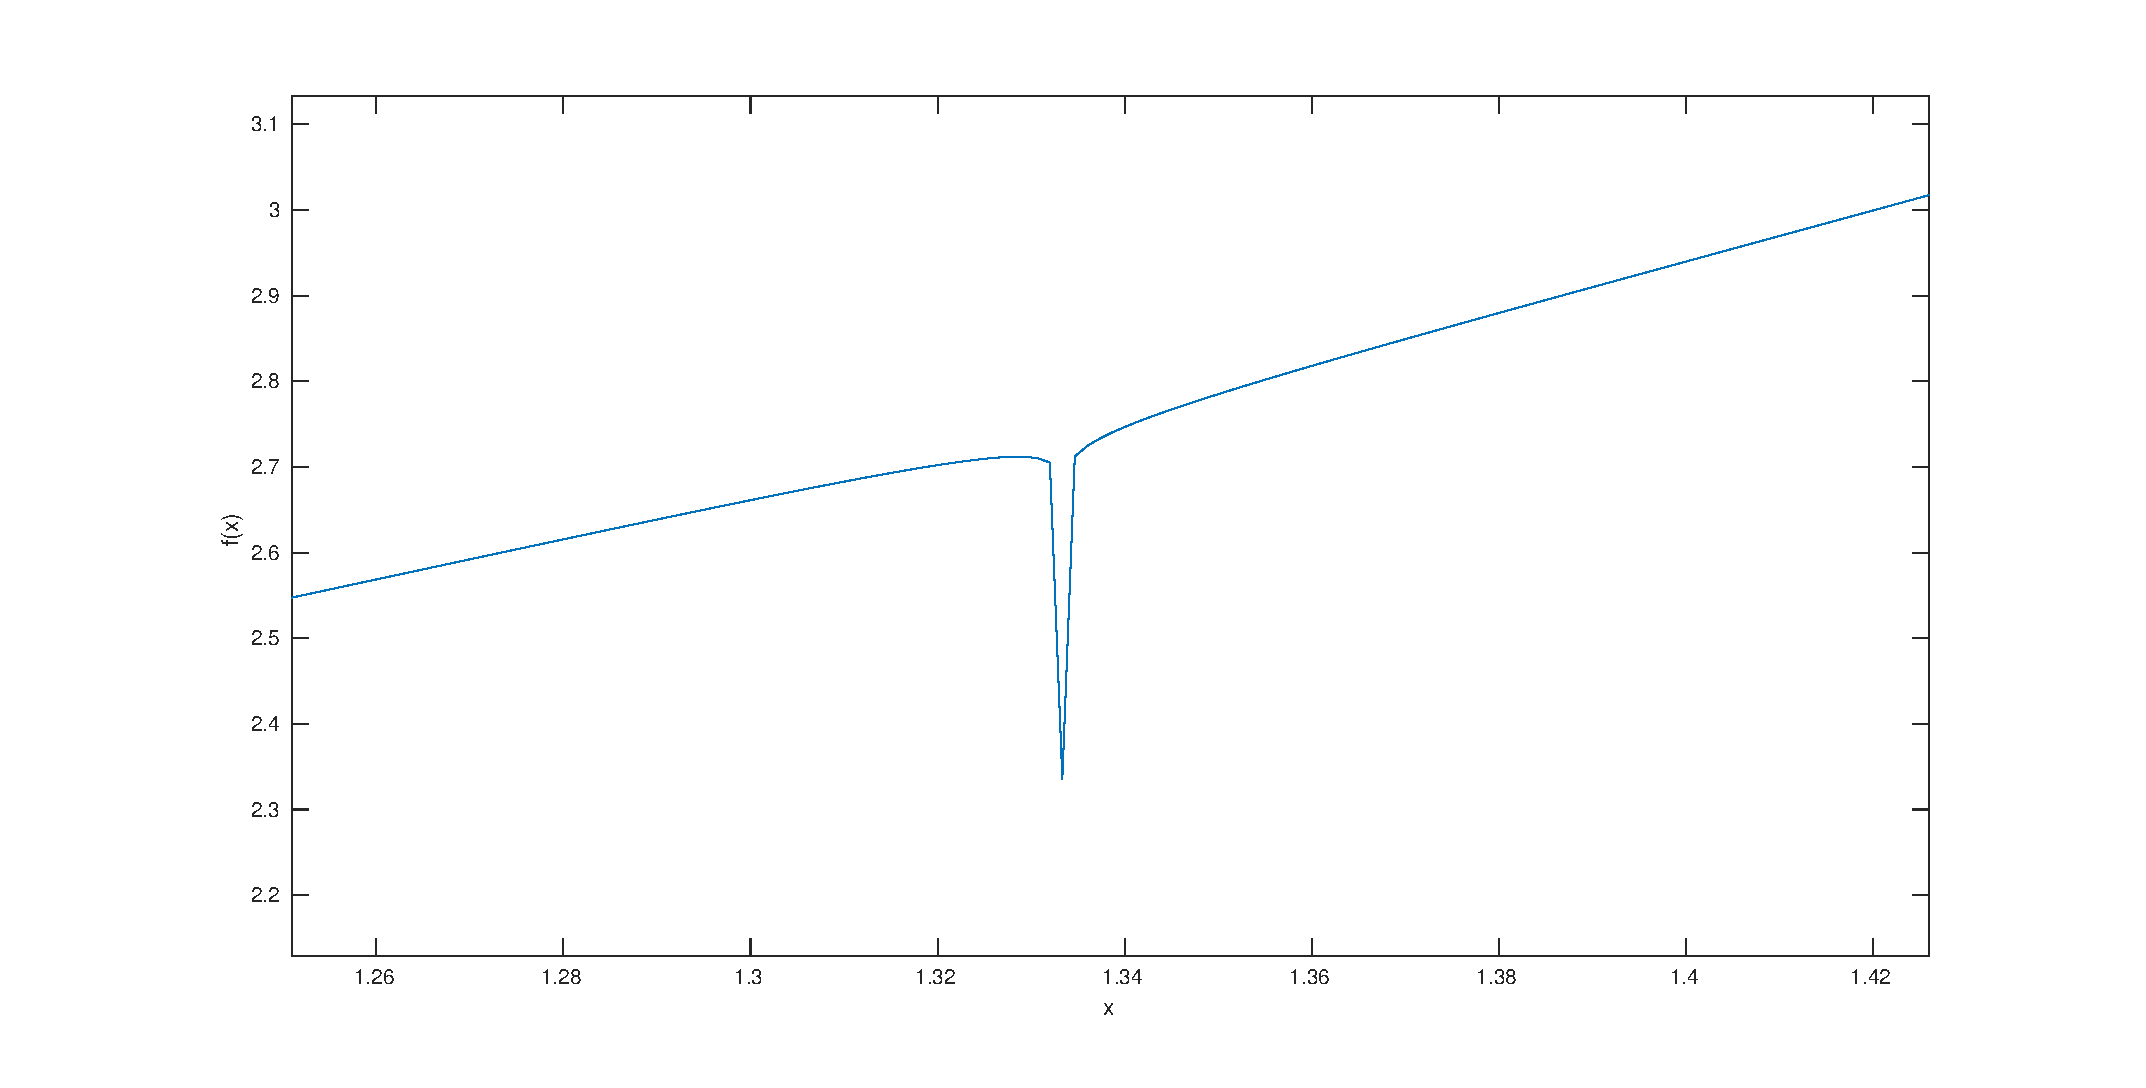
\includegraphics[width=450px]{plot/fes113}
\caption{\texttt{Plot MatLab della funzione $f(x)=\frac{ln(|3(1-x)+1|)}{80}+x^2+1$}}
\end{figure}
Si può notare che l'asintoto verticale in $x=\frac{4}{3}$ non viene rappresentato come tale. Il problema è che stiamo rappresentando dei numeri reali in un calcolatore, quindi la loro rappresentazione comporta delle approssimazioni. In questo caso infatti abbiamo il valore di $4/3$ che è un numero periodico, ma il calcolatore lo dovrà rappresentare con un numero di cifre finite causando un errore di rappresentazione che in questo caso risulta rilevante. Si allega sotto l'output del codice soprastante:
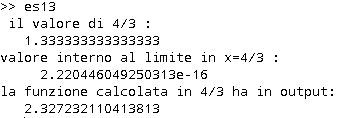
\includegraphics[width=10cm]{cap_1/es13/es113.png}
\end{flushleft}